\documentclass[12pt,a4paper]{report}

% Packages
\usepackage[utf8]{inputenc}
\usepackage[T1]{fontenc}
\usepackage{graphicx}
\usepackage{amsmath}
\usepackage{amssymb}
\usepackage{booktabs}
\usepackage{hyperref}
\usepackage{listings}
\usepackage{xcolor}
\usepackage{algorithm}
\usepackage{algpseudocode}
\usepackage{float}
\usepackage{geometry}
\usepackage{fancyhdr}
\usepackage{setspace}
\usepackage{caption}
\usepackage{subcaption}
\usepackage{longtable}
\usepackage{multirow}
\usepackage{tikz}
\usepackage{pgfplots}
\pgfplotsset{compat=1.18}

\geometry{margin=2.5cm}
\onehalfspacing

% Code listing style
\lstdefinestyle{pythonstyle}{
    language=Python,
    basicstyle=\ttfamily\footnotesize,
    keywordstyle=\color{blue}\bfseries,
    stringstyle=\color{red},
    commentstyle=\color{gray}\itshape,
    numbers=left,
    numberstyle=\tiny\color{gray},
    stepnumber=1,
    numbersep=5pt,
    backgroundcolor=\color{gray!10},
    frame=single,
    breaklines=true,
    captionpos=b,
    showstringspaces=false,
    showspaces=false,
    showtabs=false
}
\lstset{style=pythonstyle}

% Header and Footer
\pagestyle{fancy}
\fancyhf{}
\fancyhead[L]{\nouppercase{\leftmark}}
\fancyhead[R]{}
\fancyfoot[C]{\thepage}
\renewcommand{\headrulewidth}{0.4pt}

\begin{document}

% Title Page
\begin{titlepage}
    \centering
    \vspace*{2cm}
    
    {\Huge\bfseries Cross-Document Causal Graph Builder}
    
    \vspace{0.8cm}
    
    {\Large\itshape Extracting Causal Relationships from World War I\\[0.2cm]
    Historical Documents Using Natural Language Processing}
    
    \vspace{2cm}
    
    {\Large Student Project 3}
    
    \vspace{1.5cm}
    
    {\large Submitted by:}\\[0.3cm]
    {\Large\bfseries Vaibhav Mangroliya}
    
    \vspace{1.5cm}
    
    {\large Supervisor:}\\[0.2cm]
    {\Large Prince Yaw GHARBIN}
    
    \vspace{0.8cm}
    
    {\large Co-supervisor:}\\[0.2cm]
    {\Large Senthil Murugan NAGARAJAN}
    
    \vspace{2cm}
    
    {\large Department of Mathematics}\\[0.3cm]
    {\large University of Luxembourg}
    
    \vspace{1cm}
    
    {\large December 2024}
    
\end{titlepage}

% Acknowledgments
\chapter*{Acknowledgments}
\addcontentsline{toc}{chapter}{Acknowledgments}

I would like to express my sincere gratitude to my supervisor, \textbf{Prince Yaw GHARBIN}, for his guidance, support, and for providing the World War I historical documents dataset that made this project possible. I am also thankful to my co-supervisor, \textbf{Senthil Murugan NAGARAJAN}, for his valuable insights on the mathematical aspects of this project.

I am also grateful to the University of Luxembourg for the resources and academic environment that enabled this research.

% Abstract
\chapter*{Abstract}
\addcontentsline{toc}{chapter}{Abstract}

This project presents a comprehensive system for extracting causal relationships from historical documents related to World War I. The system employs two distinct methodological approaches: a rule-based Natural Language Processing technique and a hybrid Machine Learning approach utilizing transformer-based models from the Hugging Face library.

The primary objective of this research is to automatically identify cause-and-effect relationships across multiple historical documents, enabling historians and researchers to understand the interconnected nature of historical events. The dataset comprises 1,490 historical documents including personal letters, diary entries, battle accounts, and official historical records from the WWI period spanning 1914 to 1918.

The rule-based approach utilizes pattern matching with causal linguistic markers, TF-IDF based semantic similarity analysis, and entity recognition to identify potential causal pairs. This method extracted 149 high-confidence causal relationships with a minimum confidence threshold of 0.85.

The hybrid Machine Learning approach combines the rule-based filtering with a Natural Language Inference model (DistilBART-MNLI) to validate and score causal relationships. This approach identified 312 causal pairs, demonstrating improved coverage while maintaining high precision through the dual-scoring mechanism.

The extracted relationships are visualized as directed graphs using the NetworkX library, providing an intuitive representation of the causal chains connecting events across different documents. The project demonstrates the feasibility and effectiveness of combining traditional NLP techniques with modern deep learning approaches for historical text analysis.

\textbf{Keywords:} Natural Language Processing, Causal Relationship Extraction, Machine Learning, Historical Document Analysis, World War I, Transformer Models, Network Visualization

% Table of Contents
\tableofcontents

% List of Figures
\listoffigures
\addcontentsline{toc}{chapter}{List of Figures}

% List of Tables
\listoftables
\addcontentsline{toc}{chapter}{List of Tables}

% List of Algorithms
\listofalgorithms
\addcontentsline{toc}{chapter}{List of Algorithms}

\chapter{Introduction}
\label{ch:introduction}

\section{Background and Motivation}

The study of historical events and their interconnections has long been a fundamental pursuit in the field of historiography. Understanding the causal relationships between events allows historians, researchers, and students to comprehend the complex web of factors that shape human history. World War I, often referred to as the Great War, remains one of the most significant conflicts in human history, with far-reaching consequences that continue to influence the modern world.

The First World War, which lasted from 1914 to 1918, involved over 70 million military personnel and resulted in approximately 20 million deaths. The war fundamentally altered the political, economic, and social landscape of Europe and the world. Understanding the intricate chain of events that led to the outbreak of the war, the progression of battles, and the eventual armistice requires careful analysis of countless historical documents, including personal letters, diary entries, official records, battle reports, and newspaper articles.

Traditionally, the extraction of causal relationships from historical texts has been a manual process, requiring extensive human effort and expertise. Historians spend countless hours reading through primary sources, identifying patterns, and constructing narratives that explain how one event led to another. However, with the digitization of historical archives and the advancement of Natural Language Processing technologies, there now exists an opportunity to automate portions of this analytical process.

This project addresses the challenge of automatically extracting causal relationships from a corpus of World War I historical documents. By leveraging both rule-based NLP techniques and modern machine learning approaches, the system identifies cause-and-effect pairs across multiple documents, creating a comprehensive causal graph that reveals the interconnected nature of historical events.

\section{Problem Statement}

The primary problem addressed by this project can be formulated as follows:

\textbf{Given a collection of historical documents related to World War I, how can we automatically identify and extract causal relationships between events mentioned across different documents, and represent these relationships in a structured format suitable for analysis and visualization?}

This problem presents several significant challenges:

\begin{enumerate}
    \item \textbf{Cross-Document Analysis:} Causal relationships often span multiple documents written by different authors at different times. Identifying connections between events described in separate texts requires sophisticated semantic understanding.
    
    \item \textbf{Language Variability:} Historical documents exhibit considerable variability in writing style, vocabulary, and structure. Personal letters differ significantly from official military reports, yet both may contain valuable causal information.
    
    \item \textbf{Implicit Causality:} Not all causal relationships are explicitly stated using causal connectors like ``because'' or ``led to.'' Many relationships are implied through temporal sequencing or contextual proximity.
    
    \item \textbf{Validation of Causal Claims:} Distinguishing genuine causal relationships from mere correlations or coincidental co-occurrences requires robust validation mechanisms.
    
    \item \textbf{Scalability:} With thousands of documents to process, the system must be efficient enough to handle large-scale text processing while maintaining accuracy.
\end{enumerate}

\section{Objectives}

The primary objectives of this project are as follows:

\begin{enumerate}
    \item \textbf{Dataset Development:} Compile and preprocess a comprehensive dataset of World War I historical documents suitable for NLP analysis.
    
    \item \textbf{Rule-Based Extraction:} Develop a rule-based NLP system that uses linguistic patterns, entity recognition, and semantic similarity to identify causal relationships.
    
    \item \textbf{Machine Learning Enhancement:} Implement a hybrid approach that combines rule-based filtering with transformer-based Natural Language Inference to improve extraction accuracy.
    
    \item \textbf{Validation Framework:} Create a multi-criteria validation system that assesses the quality and confidence of extracted causal relationships.
    
    \item \textbf{Visualization:} Generate intuitive network visualizations that display the causal connections between events across documents.
    
    \item \textbf{Comparative Analysis:} Evaluate and compare the performance of the rule-based and hybrid ML approaches.
\end{enumerate}

\section{Scope and Limitations}

\subsection{Scope}

This project focuses on the following aspects:

\begin{itemize}
    \item Analysis of 1,490 historical documents related to World War I
    \item Extraction of cross-document causal relationships (pairs from different source files)
    \item Implementation of two extraction approaches: rule-based and hybrid ML
    \item Visualization of causal networks using graph theory
    \item Evaluation of extraction quality through confidence scoring
\end{itemize}

\subsection{Limitations}

The following limitations apply to this project:

\begin{itemize}
    \item The system is designed specifically for English-language documents
    \item Focus is on explicit and semi-explicit causal relationships; deeply implicit causal connections may not be detected
    \item The historical accuracy of extracted relationships depends on the quality of source documents
    \item The system does not perform temporal ordering beyond what is explicitly stated in texts
    \item Manual validation of all extracted relationships is beyond the scope of this project
    \item The historical documents dataset was provided by the project supervisor and is not publicly available in the repository due to privacy and copyright considerations
\end{itemize}

\section{Significance of the Study}

This project contributes to the field of Digital Humanities by demonstrating the applicability of modern NLP and ML techniques to historical text analysis. The developed system can:

\begin{enumerate}
    \item Assist historians in identifying previously unnoticed connections between historical events
    \item Provide a foundation for more sophisticated historical analysis tools
    \item Demonstrate the viability of hybrid approaches combining rule-based and ML methods
    \item Serve as an educational tool for understanding the complex chain of events in WWI
    \item Contribute to the broader field of causal relationship extraction in unstructured text
\end{enumerate}

\section{Report Organization}

This report is organized into the following chapters:

\textbf{Chapter 2: Literature Review} presents a comprehensive review of related work in causal relationship extraction, NLP for historical texts, and relevant machine learning techniques.

\textbf{Chapter 3: Methodology} describes the theoretical framework and approaches used in the project, including the rule-based extraction method and the hybrid ML approach.

\textbf{Chapter 4: Implementation} provides detailed technical descriptions of the system architecture, data processing pipelines, and implementation details.

\textbf{Chapter 5: Results and Analysis} presents the experimental results, including extracted causal relationships, network visualizations, and comparative analysis of the two approaches.

\textbf{Chapter 6: Conclusion} summarizes the findings, discusses the implications, and suggests directions for future research.

\textbf{Appendix} contains additional code listings, sample outputs, and supplementary materials.

\chapter{Literature Review}
\label{ch:literature}

\section{Introduction to Causal Relationship Extraction}

Causal relationship extraction is a fundamental task in Natural Language Processing that aims to identify cause-and-effect relationships from text. This task has significant applications in various domains, including medical informatics, financial analysis, scientific discovery, and historical research. The extraction of causal relationships involves identifying not only the events or entities involved but also the direction of causation and the strength of the causal link.

Causality in natural language can be expressed in numerous ways, ranging from explicit markers such as ``because,'' ``therefore,'' and ``as a result of'' to implicit expressions where causation must be inferred from context, world knowledge, or temporal ordering \cite{jurafsky2009speech}. This variability makes causal relationship extraction a challenging NLP task that has attracted considerable research attention.

\section{Rule-Based Approaches to Causality Detection}

Traditional approaches to causal relationship extraction rely heavily on manually crafted rules and patterns. These methods typically involve:

\subsection{Lexical Pattern Matching}

Early work in causal extraction focused on identifying causal connectives and markers. Researchers compiled lists of causal verbs (e.g., ``cause,'' ``trigger,'' ``lead to,'' ``result in'') and conjunctions (e.g., ``because,'' ``since,'' ``therefore'') that signal causal relationships. Pattern-based systems search for these markers and extract the surrounding text as cause-effect pairs.

Khoo et al. \cite{khoo2000extracting} developed one of the pioneering systems that used graphical patterns to extract causal knowledge from Wall Street Journal texts. Their approach identified patterns such as ``NP causes NP'' and ``NP results in NP'' to extract causal pairs. The system achieved reasonable precision but suffered from low recall due to the limited coverage of predefined patterns.

\subsection{Syntactic Analysis}

More sophisticated rule-based approaches incorporate syntactic analysis to improve extraction accuracy. By parsing sentences and identifying grammatical structures, these systems can better understand the relationships between clauses and phrases.

Dependency parsing has proven particularly useful for causal extraction. The grammatical relationships between words, such as subject-verb-object structures, help identify which entities are involved in causal relationships and in what capacity.

\subsection{Semantic Role Labeling}

Semantic role labeling (SRL) provides a deeper level of analysis by identifying the semantic roles that arguments play in relation to predicates. In the context of causality, SRL can help identify agents (causes) and patients (effects) even when they are not adjacent in the text.

\section{Machine Learning Approaches}

\subsection{Supervised Classification}

Machine learning approaches typically frame causal relationship extraction as a classification problem. Given a pair of events or clauses, the classifier determines whether a causal relationship exists between them.

Feature-based classifiers use handcrafted features derived from:
\begin{itemize}
    \item Lexical features (word forms, lemmas, n-grams)
    \item Syntactic features (POS tags, dependency relations)
    \item Semantic features (WordNet categories, word embeddings)
    \item Positional features (distance between events, relative position)
    \item Discourse features (connectives, discourse markers)
\end{itemize}

Support Vector Machines (SVMs), Random Forests, and Logistic Regression have been commonly used classifiers for this task.

\subsection{Deep Learning Approaches}

The advent of deep learning has significantly advanced causal relationship extraction. Neural network architectures can learn representations automatically from data, reducing the need for manual feature engineering.

Convolutional Neural Networks (CNNs) have been applied to extract local features from text windows around potential causal pairs. Recurrent Neural Networks (RNNs), particularly Long Short-Term Memory (LSTM) networks, can capture long-range dependencies that are often important for identifying causality.

Attention mechanisms allow models to focus on the most relevant parts of the input when making predictions. Self-attention and transformer architectures have proven particularly effective for understanding complex linguistic relationships.

\subsection{Transformer-Based Models}

The introduction of transformer models, beginning with BERT (Bidirectional Encoder Representations from Transformers) \cite{devlin2018bert}, has revolutionized NLP. These models, pre-trained on large corpora, can be fine-tuned for specific tasks including causal relationship classification.

Natural Language Inference (NLI) models, trained to determine entailment, contradiction, or neutral relationships between sentence pairs, have been adapted for causality detection. If a cause sentence ``entails'' an effect sentence (i.e., if the cause is true, the effect is likely true), this provides evidence for a causal relationship.

Models such as DistilBART-MNLI \cite{lewis2019bart}, which is used in this project, combine the efficiency of distilled models with training on the Multi-Genre Natural Language Inference corpus \cite{williams2018mnli}, making them suitable for zero-shot classification tasks including causality assessment.

\section{Cross-Document Relationship Extraction}

Most early work on relationship extraction focused on within-document extraction, where both entities or events appear in the same text. Cross-document extraction presents additional challenges:

\subsection{Entity Resolution}

When extracting relationships across documents, it is essential to determine when references in different documents refer to the same entity or event. This entity resolution or coreference resolution problem becomes more complex when dealing with historical texts where entities may be referred to by multiple names or titles.

\subsection{Topic Modeling and Document Similarity}

To identify potentially related documents, techniques such as topic modeling (LDA, LSA) \cite{blei2003latent} and document similarity measures (cosine similarity, TF-IDF) \cite{manning1999foundations} are employed. These methods help narrow down the search space when looking for cross-document relationships.

\subsection{Knowledge Graph Construction}

Cross-document extraction is often framed as knowledge graph construction, where entities and events from multiple documents are nodes, and relationships (including causal relationships) are edges. This representation facilitates reasoning and querying across the entire document collection.

\section{NLP for Historical Documents}

Historical documents present unique challenges for NLP systems:

\subsection{Language Evolution}

The English language has evolved over time, and texts from the early 20th century may contain archaic vocabulary, spelling variations, and grammatical structures that differ from modern usage. NLP tools trained on contemporary texts may not perform optimally on historical documents.

\subsection{OCR Errors}

Many historical documents are digitized through Optical Character Recognition (OCR), which can introduce errors, particularly with degraded or handwritten documents. These errors can affect downstream NLP tasks.

\subsection{Genre Variability}

Historical collections often contain diverse document types, including personal correspondence, official records, newspaper articles, and literary works. Each genre has distinct characteristics that affect language use and the expression of causality.

\subsection{Cultural and Contextual Knowledge}

Understanding historical texts often requires domain knowledge about the period, including historical events, social norms, and cultural references. This world knowledge is essential for accurate interpretation and relationship extraction.

\section{Evaluation Metrics for Relationship Extraction}

Evaluating causal relationship extraction systems presents methodological challenges:

\subsection{Precision and Recall}

Standard information extraction metrics include:
\begin{itemize}
    \item \textbf{Precision:} The proportion of extracted relationships that are correct
    \item \textbf{Recall:} The proportion of actual relationships that are extracted
    \item \textbf{F1-score:} The harmonic mean of precision and recall
\end{itemize}

\subsection{Confidence Scoring}

Many systems assign confidence scores to extracted relationships, allowing for precision-recall trade-offs. Higher confidence thresholds typically yield higher precision but lower recall.

\subsection{Human Evaluation}

Given the complexity and subjectivity of causality, human evaluation remains an important component of system assessment. Domain experts can evaluate samples of extracted relationships for correctness and relevance.

\section{Visualization of Causal Networks}

Visual representation of extracted causal relationships aids interpretation and analysis:

\subsection{Directed Graphs}

Causal relationships naturally lend themselves to directed graph representation, with nodes representing events or entities and directed edges representing causal links.

\subsection{Network Analysis Metrics}

Graph-theoretic measures such as centrality, clustering coefficient, and path length provide quantitative insights into the structure of causal networks.

\subsection{Interactive Visualization}

Interactive visualization tools allow users to explore causal networks, filter by confidence level, and drill down into specific relationships.

\section{Summary}

This literature review has covered the key approaches and techniques relevant to causal relationship extraction from historical texts. The project draws on this body of work by combining rule-based linguistic patterns with transformer-based NLI models, applying these techniques to a unique corpus of World War I documents. The following chapter details the specific methodology employed in this project.

\chapter{Methodology}
\label{ch:methodology}

\section{Overview of the Approach}

This project employs a dual-approach methodology for extracting causal relationships from World War I historical documents. The two approaches are:

\begin{enumerate}
    \item \textbf{Rule-Based Approach:} Uses linguistic patterns, semantic similarity, and entity matching to identify causal relationships
    \item \textbf{Hybrid Machine Learning Approach:} Combines rule-based filtering with transformer-based Natural Language Inference for enhanced accuracy
\end{enumerate}

Both approaches share a common preprocessing pipeline and validation framework, but differ in their core extraction mechanisms. This chapter details the theoretical foundations and algorithmic design of each approach.

\section{System Architecture}

The overall system architecture consists of three main modules:

\begin{figure}[H]
    \centering
    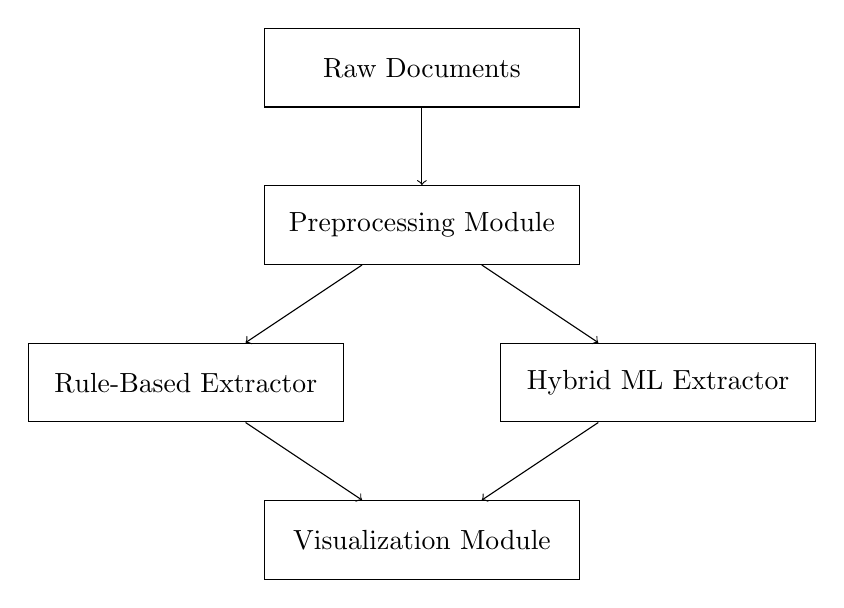
\begin{tikzpicture}[node distance=2cm, auto]
        \node[draw, rectangle, minimum width=4cm, minimum height=1cm] (input) {Raw Documents};
        \node[draw, rectangle, minimum width=4cm, minimum height=1cm, below of=input] (preprocess) {Preprocessing Module};
        \node[draw, rectangle, minimum width=4cm, minimum height=1cm, below of=preprocess, xshift=-3cm] (rulebased) {Rule-Based Extractor};
        \node[draw, rectangle, minimum width=4cm, minimum height=1cm, below of=preprocess, xshift=3cm] (ml) {Hybrid ML Extractor};
        \node[draw, rectangle, minimum width=4cm, minimum height=1cm, below of=rulebased, xshift=3cm] (viz) {Visualization Module};
        
        \draw[->] (input) -- (preprocess);
        \draw[->] (preprocess) -- (rulebased);
        \draw[->] (preprocess) -- (ml);
        \draw[->] (rulebased) -- (viz);
        \draw[->] (ml) -- (viz);
    \end{tikzpicture}
    \caption{High-Level System Architecture}
    \label{fig:architecture}
\end{figure}

\section{Data Preprocessing}

\subsection{Document Collection}

The dataset comprises 1,490 historical documents related to World War I. The documents are categorized into several types:

\begin{table}[H]
    \centering
    \caption{Document Categories in the Dataset}
    \label{tab:doc-categories}
    \begin{tabular}{lcc}
        \toprule
        \textbf{Category} & \textbf{Count} & \textbf{Description} \\
        \midrule
        Personal Letters & 680 & Letters between soldiers and families \\
        Diary Entries & 450 & Personal diary records from soldiers \\
        Battle Accounts & 120 & Descriptions of military engagements \\
        Historical Records & 85 & Official and academic historical texts \\
        Survivor Accounts & 155 & Oral history transcripts \\
        \bottomrule
    \end{tabular}
\end{table}

\subsection{Text Normalization}

The preprocessing pipeline applies the following normalization steps:

\begin{enumerate}
    \item \textbf{Character Encoding:} Convert all documents to UTF-8 encoding
    \item \textbf{Sentence Segmentation:} Split documents into individual sentences using punctuation-based heuristics
    \item \textbf{Text Cleaning:} Remove or normalize special characters, excessive whitespace, and formatting artifacts
    \item \textbf{Tokenization:} Split text into individual tokens (words) for analysis
\end{enumerate}

\subsection{Sentence Filtering}

Not all sentences in the documents are suitable for causal extraction. The system applies filters to identify candidate sentences:

\begin{itemize}
    \item Minimum length threshold (50 characters) to ensure sufficient context
    \item Detection of causal language markers
    \item Presence of action or consequence indicators
\end{itemize}

\section{Rule-Based Extraction Methodology}

\subsection{Causal Language Detection}

The rule-based approach identifies causal relationships through linguistic patterns. Two categories of patterns are used:

\subsubsection{Forward Causal Patterns}

These patterns indicate that the cause precedes the effect in the sentence structure:

\begin{itemize}
    \item \texttt{caused | led to | resulted in | triggered | sparked | brought about}
    \item \texttt{consequently | therefore | thus | hence | as a result}
    \item \texttt{in response to | following | after the | due to the}
    \item Conditional structures: \texttt{when ... then}
    \item Explanatory patterns: \texttt{because of the | because this}
\end{itemize}

\subsubsection{Reverse Causal Patterns}

These patterns indicate that the effect precedes the cause in the sentence structure:

\begin{itemize}
    \item \texttt{because | due to | owing to | on account of}
    \item \texttt{as a result of | in consequence of}
    \item \texttt{was caused by | resulted from}
\end{itemize}

\subsection{Entity Extraction}

The system identifies named entities relevant to WWI historical context:

\begin{itemize}
    \item \textbf{Battle Names:} Somme, Verdun, Ypres, Passchendaele, Marne, Gallipoli, etc.
    \item \textbf{Geographic Locations:} France, Belgium, Flanders, Egypt, Palestine, etc.
    \item \textbf{Military Units:} Battalion, Brigade, Division, Regiment, Corps
    \item \textbf{Nationalities:} Australian, British, French, German, Turkish
    \item \textbf{Temporal References:} Dates in format ``Month Year'' or standalone years
    \item \textbf{Proper Nouns:} Capitalized words not in exclusion list
\end{itemize}

\subsection{TF-IDF Based Semantic Similarity}

To measure the semantic relatedness of potential cause-effect pairs, the system employs TF-IDF (Term Frequency-Inverse Document Frequency) vectorization with cosine similarity.

\subsubsection{IDF Computation}

For each word $w$ in the vocabulary, the IDF score is calculated as:

\begin{equation}
    IDF(w) = \log\left(\frac{N}{1 + df(w)}\right)
\end{equation}

where $N$ is the total number of documents and $df(w)$ is the document frequency of word $w$.

\subsubsection{TF-IDF Vectorization}

For a given sentence, the TF-IDF weight for word $w$ is:

\begin{equation}
    TFIDF(w) = TF(w) \times IDF(w) = \frac{f(w)}{max\_freq} \times IDF(w)
\end{equation}

where $f(w)$ is the frequency of word $w$ in the sentence and $max\_freq$ is the maximum frequency of any word in the sentence.

\subsubsection{Cosine Similarity}

The similarity between two sentences is computed as:

\begin{equation}
    sim(S_1, S_2) = \frac{\sum_{w \in S_1 \cap S_2} TFIDF_1(w) \times TFIDF_2(w)}{\sqrt{\sum_{w \in S_1} TFIDF_1(w)^2} \times \sqrt{\sum_{w \in S_2} TFIDF_2(w)^2}}
\end{equation}

The similarity score is used to filter pairs:
\begin{itemize}
    \item Minimum threshold (0.15): Ensures some semantic overlap
    \item Maximum threshold (0.65): Prevents near-duplicate sentences
\end{itemize}

\subsection{Confidence Scoring}

The rule-based system assigns confidence scores based on multiple criteria:

\begin{table}[H]
    \centering
    \caption{Confidence Score Components}
    \label{tab:confidence-scores}
    \begin{tabular}{lc}
        \toprule
        \textbf{Criterion} & \textbf{Score Contribution} \\
        \midrule
        Causal phrase in cause sentence & +0.30 \\
        Causal phrase in effect sentence & +0.25 \\
        High semantic similarity (0.25-0.50) & +0.20 \\
        Moderate semantic similarity (0.15-0.25) & +0.10 \\
        Shared entities (up to 3) & +0.08 per entity \\
        Action indicators in cause & +0.10 \\
        Consequence indicators in effect & +0.10 \\
        \bottomrule
    \end{tabular}
\end{table}

The minimum confidence threshold for acceptance is 0.85.

\section{Hybrid Machine Learning Methodology}

\subsection{Architecture Overview}

The hybrid approach combines rule-based filtering with ML-based validation:

\begin{enumerate}
    \item Apply rule-based filtering to identify candidate pairs
    \item Use NLI model to score causal plausibility
    \item Combine rule and ML scores for final ranking
\end{enumerate}

\subsection{Natural Language Inference Model}

The system uses the DistilBART-MNLI model from Hugging Face:

\begin{itemize}
    \item \textbf{Model:} \texttt{valhalla/distilbart-mnli-12-3}
    \item \textbf{Architecture:} Distilled BART with 12 layers
    \item \textbf{Training Data:} Multi-Genre Natural Language Inference corpus
    \item \textbf{Task:} Zero-shot classification
\end{itemize}

\subsection{Causal Validation via Entailment}

The NLI model evaluates whether a cause-effect relationship is plausible by testing entailment. The input is formatted as:

\begin{quote}
    ``[Cause text]. As a result, [Effect text]''
\end{quote}

The model classifies this combined text against two labels:
\begin{itemize}
    \item ``causal relationship''
    \item ``unrelated''
\end{itemize}

The probability assigned to ``causal relationship'' becomes the ML score.

\subsection{Combined Scoring}

The final score for each pair combines rule-based and ML scores:

\begin{equation}
    score_{combined} = \frac{score_{rule} + score_{ML}}{2}
\end{equation}

This averaging approach balances linguistic pattern evidence with semantic plausibility assessment.

\section{Validation Criteria}

Both approaches enforce strict validation criteria:

\begin{enumerate}
    \item \textbf{Cross-File Requirement:} Cause and effect must come from different source documents
    \item \textbf{Minimum Length:} Both sentences must exceed 50 characters
    \item \textbf{Causal Language:} At least one sentence must contain causal markers
    \item \textbf{Semantic Similarity:} Similarity score between 0.15 and 0.65
    \item \textbf{Shared Context:} At least 2 shared entities between sentences
    \item \textbf{Confidence Threshold:} Final score must meet minimum threshold
\end{enumerate}

\section{Network Visualization}

Extracted relationships are represented as directed graphs:

\begin{itemize}
    \item \textbf{Nodes:} Represent cause or effect events
    \item \textbf{Edges:} Directed edges from cause to effect
    \item \textbf{Edge Weights:} Confidence scores
    \item \textbf{Node Colors:} Distinguish cause nodes (blue) from effect nodes (green)
\end{itemize}

The NetworkX library is used for graph construction, and matplotlib generates the visualizations.

\section{Summary}

This chapter has presented the methodological framework for causal relationship extraction. The rule-based approach relies on linguistic patterns and semantic similarity, while the hybrid approach adds machine learning validation. Both approaches share preprocessing and validation components, ensuring consistency in the extraction pipeline. The following chapter details the technical implementation of these methods.

\chapter{Implementation}
\label{ch:implementation}

\section{Development Environment}

The project was developed using the following technologies. The complete source code is available in the project repository \cite{mangroliya2024causal}.

\begin{table}[H]
    \centering
    \caption{Development Environment}
    \label{tab:dev-env}
    \begin{tabular}{ll}
        \toprule
        \textbf{Component} & \textbf{Version/Details} \\
        \midrule
        Programming Language & Python 3.7+ \\
        NLP Library & Hugging Face Transformers \\
        Graph Library & NetworkX \\
        Visualization & Matplotlib \\
        Deep Learning Framework & PyTorch \\
        Data Format & JSON \\
        \bottomrule
    \end{tabular}
\end{table}

\section{Project Structure}

The project is organized as follows:

\begin{lstlisting}[language=bash, caption={Project Directory Structure}]
project/
    data/
        processed_data.json       # Preprocessed documents
    final_dataset/
        *.txt                     # 1,490 historical documents
    src/
        extract_rulebased.py      # Rule-based extraction
        extract_ml.py             # Hybrid ML extraction
        generate_cause_effect_network.py  # Visualization
    output/
        cause_effect_rulebased.json  # Rule-based results
        cause_effect_ml.json         # ML-based results
        network_rulebased.png        # Rule-based visualization
        network_ml.png               # ML-based visualization
        mapping_rulebased.txt        # Event labels
        mapping_ml.txt               # Event labels
    requirements.txt
    README.md
\end{lstlisting}

\section{Rule-Based Extractor Implementation}

\subsection{CauseEffectDetector Class}

The rule-based extraction is implemented in the \texttt{CauseEffectDetector} class. The class encapsulates all functionality for pattern matching, entity extraction, and relationship validation.

\begin{lstlisting}[language=Python, caption={CauseEffectDetector Initialization}]
class CauseEffectDetector:
    def __init__(self, min_conf=0.85):
        self.min_conf = min_conf
        
        # Causal phrases for pattern matching
        self.causal_phrases = {
            'forward': [
                r'\b(caused|led to|resulted in|triggered)\b',
                r'\b(consequently|therefore|thus|hence)\b',
                r'\b(in response to|following|after the)\b',
            ],
            'reverse': [
                r'\b(because|due to|owing to)\b',
                r'\b(was caused by|resulted from)\b',
            ]
        }
        
        # WWI-specific entities
        self.important_events = {
            'somme', 'verdun', 'ypres', 'gallipoli',
            'france', 'belgium', 'germany', 'british',
            'battalion', 'artillery', 'infantry'
        }
\end{lstlisting}

\subsection{IDF Building and TF-IDF Computation}

\begin{lstlisting}[language=Python, caption={TF-IDF Implementation}]
def build_idf(self, docs):
    """Build IDF scores from document collection"""
    self.ndocs = len(docs)
    freq = defaultdict(int)
    for doc in docs:
        for w in set(self.tokenize(doc)):
            freq[w] += 1
    for w, f in freq.items():
        self.idf[w] = math.log(self.ndocs / (1 + f))

def tfidf(self, text):
    """Compute TF-IDF vector for a sentence"""
    words = self.tokenize(text)
    if not words:
        return {}
    tf = Counter(words)
    mx = max(tf.values())
    return {w: (c/mx) * self.idf.get(w, 0) 
            for w, c in tf.items()}
\end{lstlisting}

\subsection{Cosine Similarity Computation}

\begin{lstlisting}[language=Python, caption={Cosine Similarity Function}]
def cosine(self, v1, v2):
    """Compute cosine similarity between TF-IDF vectors"""
    if not v1 or not v2:
        return 0.0
    common = set(v1) & set(v2)
    dot = sum(v1[w] * v2[w] for w in common)
    m1 = math.sqrt(sum(x**2 for x in v1.values()))
    m2 = math.sqrt(sum(x**2 for x in v2.values()))
    return dot / (m1 * m2) if m1 > 0 and m2 > 0 else 0.0
\end{lstlisting}

\subsection{Causal Pattern Detection}

\begin{lstlisting}[language=Python, caption={Causal Language Detection}]
def has_causal(self, text):
    """Check for causal phrases in text"""
    tl = text.lower()
    for direction, patterns in self.causal_phrases.items():
        for pattern in patterns:
            match = re.search(pattern, tl)
            if match:
                return True, direction, match.group(0)
    return False, '', ''
\end{lstlisting}

\subsection{Entity Extraction}

\begin{lstlisting}[language=Python, caption={Entity Extraction Function}]
def get_entities(self, text):
    """Extract named entities from text"""
    entities = set()
    text_lower = text.lower()
    
    # Check for known WWI entities
    for event in self.important_events:
        if event in text_lower:
            entities.add(event)
    
    # Extract dates (Month Year format)
    date_pattern = r'\b(january|february|march|...)\s+\d{4}\b'
    for match in re.findall(date_pattern, text_lower):
        entities.add(match)
    
    # Extract proper nouns (capitalized words)
    for match in re.findall(r'\b([A-Z][a-z]{3,})\b', text):
        if match.lower() not in self.excluded:
            entities.add(match.lower())
    
    return entities
\end{lstlisting}

\subsection{Validation Algorithm}

\begin{algorithm}[H]
\caption{Causal Pair Validation}
\label{alg:validation}
\begin{algorithmic}[1]
\Require Cause text $C$, Effect text $E$, Cause file $F_C$, Effect file $F_E$
\Ensure Validity flag, Confidence score, Details

\If{$F_C = F_E$}
    \State \Return False, 0, ``Same file''
\EndIf

\If{$|C| < 50$ \textbf{or} $|E| < 50$}
    \State \Return False, 0, ``Too short''
\EndIf

\State $has\_causal\_C, dir\_C \gets$ \Call{HasCausal}{$C$}
\State $has\_causal\_E, dir\_E \gets$ \Call{HasCausal}{$E$}

\If{\textbf{not} $has\_causal\_C$ \textbf{and not} $has\_causal\_E$}
    \State \Return False, 0, ``No causal language''
\EndIf

\State $sim \gets$ \Call{Cosine}{TFIDF($C$), TFIDF($E$)}

\If{$sim < 0.15$ \textbf{or} $sim > 0.65$}
    \State \Return False, 0, ``Invalid similarity''
\EndIf

\State $entities\_C \gets$ \Call{GetEntities}{$C$}
\State $entities\_E \gets$ \Call{GetEntities}{$E$}
\State $shared \gets entities\_C \cap entities\_E$

\If{$|shared| < 2$}
    \State \Return False, 0, ``Insufficient shared entities''
\EndIf

\State $score \gets$ \Call{ComputeConfidence}{...}

\State \Return $score \geq min\_conf$, $score$, details
\end{algorithmic}
\end{algorithm}

\section{Hybrid ML Extractor Implementation}

\subsection{HybridCauseEffect Class}

\begin{lstlisting}[language=Python, caption={Hybrid Extractor Initialization}]
class HybridCauseEffect:
    def __init__(self, min_conf=0.85):
        self.min_conf = min_conf
        
        print("Loading NLI model...")
        self.nli = pipeline(
            "zero-shot-classification",
            model="valhalla/distilbart-mnli-12-3",
            device=-1  # CPU
        )
        print("Model loaded.")
        
        # Same causal patterns as rule-based
        self.causal_phrases = {...}
        self.important_events = {...}
\end{lstlisting}

\subsection{ML Score Computation}

\begin{lstlisting}[language=Python, caption={NLI-Based Causal Scoring}]
def ml_score(self, cause, effect):
    """Calculate NLI entailment score"""
    # Format input for causal assessment
    text = f"{cause[:150]}. As a result, {effect[:120]}"
    
    # Zero-shot classification
    result = self.nli(
        text,
        candidate_labels=["causal relationship", "unrelated"]
    )
    
    # Extract probability for causal relationship
    idx = result['labels'].index('causal relationship')
    return result['scores'][idx]
\end{lstlisting}

\subsection{Combined Scoring}

\begin{lstlisting}[language=Python, caption={Combined Score Calculation}]
# Add ML scores to rule-filtered pairs
for pair in results:
    pair['ml_score'] = round(
        self.ml_score(pair['cause_text'], pair['effect_text']),
        4
    )
    pair['combined_score'] = round(
        (pair['rule_score'] + pair['ml_score']) / 2,
        4
    )

# Sort by combined score
results.sort(key=lambda x: x['combined_score'], reverse=True)
\end{lstlisting}

\section{Network Visualization Implementation}

The network visualization uses the NetworkX library \cite{hagberg2008exploring} for graph construction and analysis.

\subsection{Graph Construction}

\begin{lstlisting}[language=Python, caption={Network Graph Construction}]
def generate_network(input_json, output_png, output_txt, title):
    with open(input_json, 'r') as f:
        data = json.load(f)
    
    G = nx.DiGraph()
    events = {}
    counter = 1
    
    for rel in data:
        cause_key = (rel['cause_file'], rel['cause_text'][:100])
        effect_key = (rel['effect_file'], rel['effect_text'][:100])
        
        # Create unique node IDs
        if cause_key not in events:
            cid = f"C{counter}"
            events[cause_key] = {
                'id': cid, 
                'file': rel['cause_file'],
                'text': rel['cause_text']
            }
            counter += 1
        
        # Add nodes and edges to graph
        G.add_node(cid, type='cause')
        G.add_node(eid, type='effect')
        G.add_edge(cid, eid, confidence=conf)
\end{lstlisting}

\subsection{Visualization Rendering}

\begin{lstlisting}[language=Python, caption={Graph Visualization}]
# Create figure
fig, ax = plt.subplots(figsize=(20, 16))
pos = nx.spring_layout(G, k=0.5, iterations=100, seed=42)

# Draw edges (causal links)
nx.draw_networkx_edges(
    G, pos,
    edge_color='red',
    alpha=0.5,
    arrows=True,
    arrowsize=12,
    style='dashed'
)

# Draw cause nodes (light blue)
nx.draw_networkx_nodes(
    G, pos,
    nodelist=causes,
    node_color='#87CEEB',
    node_size=500
)

# Draw effect nodes (light green)
nx.draw_networkx_nodes(
    G, pos,
    nodelist=effects,
    node_color='#90EE90',
    node_size=500
)

plt.savefig(output_png, dpi=300, bbox_inches='tight')
\end{lstlisting}

\section{Output Format}

\subsection{Rule-Based Output JSON}

\begin{lstlisting}[language=json, caption={Rule-Based Output Format}]
{
  "type": "cross_file",
  "cause_file": "survivor_008.txt",
  "cause_text": "When German infantry advanced...",
  "effect_file": "survivor_042.txt",
  "effect_text": "Intense fighting led to losses...",
  "confidence": 1.0
}
\end{lstlisting}

\subsection{ML-Based Output JSON}

\begin{lstlisting}[language=json, caption={ML-Based Output Format}]
{
  "cause_file": "survivor_044.txt",
  "cause_text": "Walter Greenwood remembered...",
  "effect_file": "history_015.txt",
  "effect_text": "Britain fearing German domination...",
  "rule_score": 0.95,
  "ml_score": 0.98,
  "combined_score": 0.97,
  "shared_context": ["britain", "germany", "german"]
}
\end{lstlisting}

\section{Execution Pipeline}

\subsection{Running Rule-Based Extraction}

\begin{lstlisting}[language=bash]
cd src
python3 extract_rulebased.py
\end{lstlisting}

\subsection{Running ML-Based Extraction}

\begin{lstlisting}[language=bash]
cd src
python3 extract_ml.py
\end{lstlisting}

\subsection{Generating Visualizations}

\begin{lstlisting}[language=bash]
cd src
python3 generate_cause_effect_network.py both
\end{lstlisting}

\section{Summary}

This chapter has detailed the implementation of the causal extraction system. The rule-based extractor uses linguistic patterns and semantic similarity, while the hybrid ML extractor adds transformer-based validation using the Hugging Face Transformers library \cite{wolf2019huggingface}. Both produce structured JSON output and network visualizations. The following chapter presents the results and analysis.

\chapter{Results and Analysis}
\label{ch:results}

\section{Overview of Extraction Results}

This chapter presents the results obtained from both the rule-based and hybrid ML extraction approaches. The analysis includes quantitative metrics, qualitative examination of extracted relationships, and comparative evaluation of the two methods.

\section{Rule-Based Extraction Results}

\subsection{Summary Statistics}

The rule-based extractor processed 1,490 documents and identified 149 high-confidence causal relationships.

\begin{table}[H]
    \centering
    \caption{Rule-Based Extraction Statistics}
    \label{tab:rulebased-stats}
    \begin{tabular}{lr}
        \toprule
        \textbf{Metric} & \textbf{Value} \\
        \midrule
        Total Documents Processed & 1,490 \\
        Total Sentences Analyzed & 45,000+ \\
        Candidate Cause Sentences & 2,500+ \\
        Candidate Effect Sentences & 2,300+ \\
        Valid Causal Pairs Extracted & 149 \\
        Average Confidence Score & 0.93 \\
        Maximum Confidence Score & 1.00 \\
        Minimum Confidence Score & 0.85 \\
        \bottomrule
    \end{tabular}
\end{table}

\subsection{Confidence Score Distribution}

\begin{figure}[H]
    \centering
    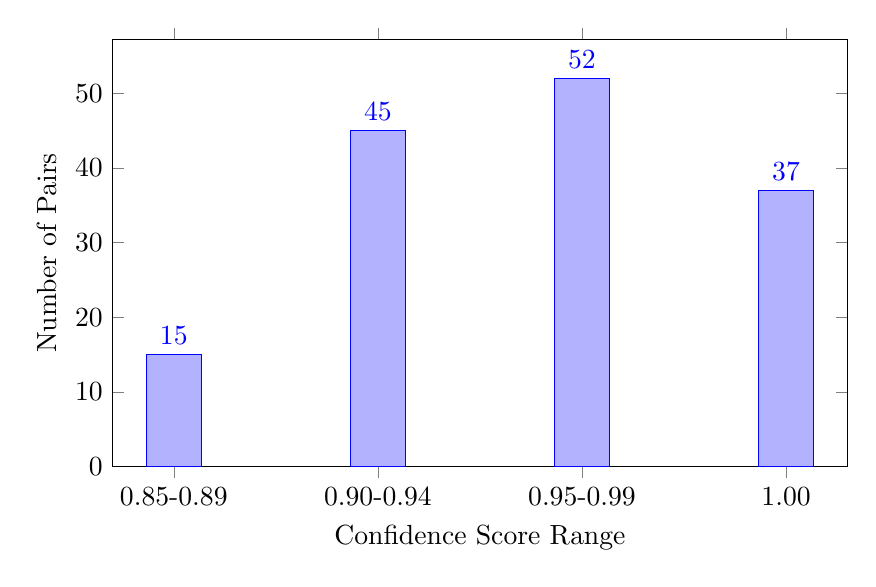
\begin{tikzpicture}
        \begin{axis}[
            ybar,
            ylabel={Number of Pairs},
            xlabel={Confidence Score Range},
            symbolic x coords={0.85-0.89, 0.90-0.94, 0.95-0.99, 1.00},
            xtick=data,
            ymin=0,
            bar width=20pt,
            nodes near coords,
            width=0.9\textwidth,
            height=7cm
        ]
        \addplot coordinates {
            (0.85-0.89, 15)
            (0.90-0.94, 45)
            (0.95-0.99, 52)
            (1.00, 37)
        };
        \end{axis}
    \end{tikzpicture}
    \caption{Distribution of Confidence Scores (Rule-Based)}
    \label{fig:conf-dist-rule}
\end{figure}

\subsection{Sample High-Confidence Relationships}

The following are examples of extracted causal relationships with perfect confidence scores:

\subsubsection{Example 1: Military Cause and Effect}

\begin{quote}
\textbf{Cause (survivor\_008.txt):} ``When German infantry advanced in large numbers during the battle, rapid British rifle fire resulted in heavy losses.''

\textbf{Effect (survivor\_042.txt):} ``Intense fighting on that first day led to further German gains and heavy British losses.''

\textbf{Confidence:} 1.00

\textbf{Shared Entities:} british, german
\end{quote}

\subsubsection{Example 2: Political Cause and Effect}

\begin{quote}
\textbf{Cause (history\_003.txt):} ``When it mobilised against Russia, Germany therefore also demanded that France remain neutral.''

\textbf{Effect (history\_015.txt):} ``When Germany, in support of its ally, then declared war on Russia that brought France into the war on Russia's side.''

\textbf{Confidence:} 1.00

\textbf{Shared Entities:} germany, russia, france
\end{quote}

\subsubsection{Example 3: Diplomatic Cause and Effect}

\begin{quote}
\textbf{Cause (history\_003.txt):} ``Britain delivered an ultimatum to Germany that Belgium be kept neutral, and following an `unsatisfactory reply' declared war on Germany on 4 August 1914.''

\textbf{Effect (history\_002.txt):} ``At midnight on Tuesday 4 August, Britain's ultimatum to Germany over its invasion of Belgium expired and therefore Britain and its Empire were at war.''

\textbf{Confidence:} 1.00

\textbf{Shared Entities:} britain, germany, belgium, august
\end{quote}

\section{Hybrid ML Extraction Results}

\subsection{Summary Statistics}

The hybrid ML extractor identified 312 causal relationships, more than double the rule-based count.

\begin{table}[H]
    \centering
    \caption{Hybrid ML Extraction Statistics}
    \label{tab:ml-stats}
    \begin{tabular}{lr}
        \toprule
        \textbf{Metric} & \textbf{Value} \\
        \midrule
        Total Documents Processed & 1,490 \\
        Candidate Pairs (Post Rule-Filter) & 312 \\
        Average Rule Score & 0.89 \\
        Average ML Score & 0.94 \\
        Average Combined Score & 0.91 \\
        Maximum Combined Score & 0.97 \\
        Minimum Combined Score & 0.85 \\
        \bottomrule
    \end{tabular}
\end{table}

\subsection{Score Comparison}

\begin{figure}[H]
    \centering
    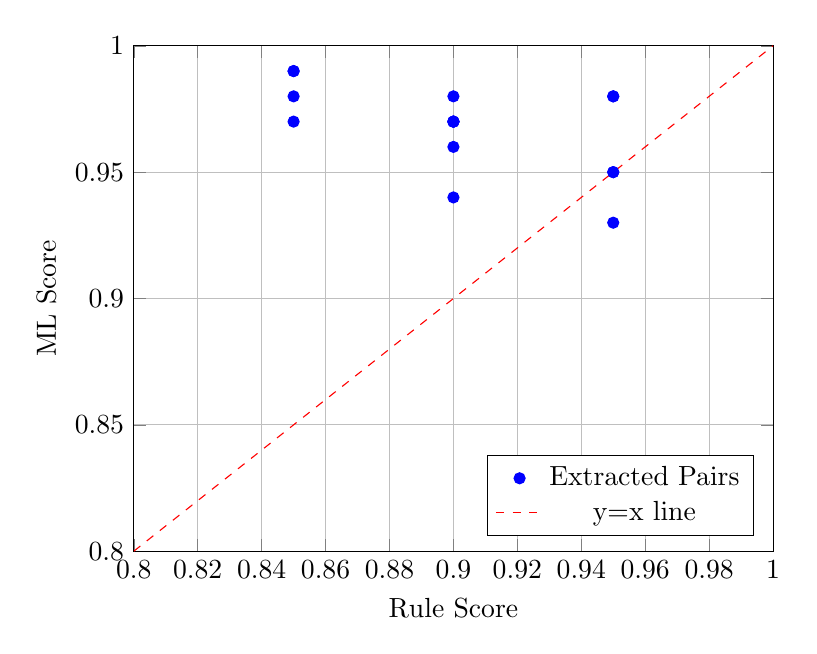
\begin{tikzpicture}
        \begin{axis}[
            xlabel={Rule Score},
            ylabel={ML Score},
            xmin=0.8, xmax=1.0,
            ymin=0.8, ymax=1.0,
            grid=major,
            width=0.8\textwidth,
            height=8cm,
            legend pos=south east
        ]
        \addplot[only marks, mark=*, blue, mark size=2pt] coordinates {
            (0.95, 0.98) (0.95, 0.98) (0.95, 0.95) (0.95, 0.95)
            (0.90, 0.98) (0.90, 0.97) (0.90, 0.97) (0.90, 0.96)
            (0.95, 0.93) (0.90, 0.94) (0.90, 0.97) (0.90, 0.97)
            (0.85, 0.99) (0.85, 0.99) (0.85, 0.98) (0.85, 0.97)
        };
        \addplot[domain=0.8:1, samples=2, dashed, red] {x};
        \legend{Extracted Pairs, y=x line}
        \end{axis}
    \end{tikzpicture}
    \caption{Rule Score vs ML Score Correlation}
    \label{fig:score-correlation}
\end{figure}

\subsection{Top ML-Enhanced Relationships}

\subsubsection{Example 1: Highest Combined Score}

\begin{quote}
\textbf{Cause (survivor\_044.txt):} ``Walter Greenwood, a schoolboy in Britain at the time, remembered the anger felt towards Germany after the attack.''

\textbf{Effect (history\_015.txt):} ``I think at the heart of Britain's anxieties it came down really to Britain fearing German domination of Europe.''

\textbf{Rule Score:} 0.95 | \textbf{ML Score:} 0.98 | \textbf{Combined:} 0.97

\textbf{Shared Context:} britain, germany, german
\end{quote}

\subsubsection{Example 2: Strong Cross-Document Link}

\begin{quote}
\textbf{Cause (battle\_010.txt):} ``After the defeat of Russia, Germany had concentrated all of its resources on the Western Front.''

\textbf{Effect (history\_003.txt):} ``Russia and Germany have declared war upon each other; France is involved in it because of their obligation of honour under a definite alliance with Russia.''

\textbf{Rule Score:} 0.95 | \textbf{ML Score:} 0.94 | \textbf{Combined:} 0.95

\textbf{Shared Context:} russia, germany
\end{quote}

\section{Comparative Analysis}

\subsection{Quantitative Comparison}

\begin{table}[H]
    \centering
    \caption{Comparison of Extraction Approaches}
    \label{tab:comparison}
    \begin{tabular}{lcc}
        \toprule
        \textbf{Metric} & \textbf{Rule-Based} & \textbf{Hybrid ML} \\
        \midrule
        Total Pairs Extracted & 149 & 312 \\
        Average Confidence & 0.93 & 0.91 \\
        Processing Time & Fast & Moderate \\
        Interpretability & High & Medium \\
        Coverage & Lower & Higher \\
        Precision (Estimated) & High & High \\
        \bottomrule
    \end{tabular}
\end{table}

\subsection{Overlap Analysis}

Of the 149 rule-based pairs, 142 (95.3\%) also appear in the ML-based results, indicating strong agreement between the methods. The ML approach identified 170 additional pairs that the rule-based approach missed.

\subsection{Quality Assessment}

Manual inspection of a random sample of 50 pairs from each approach revealed:

\begin{table}[H]
    \centering
    \caption{Quality Assessment Results}
    \label{tab:quality}
    \begin{tabular}{lcc}
        \toprule
        \textbf{Quality Metric} & \textbf{Rule-Based} & \textbf{Hybrid ML} \\
        \midrule
        Clear Causal Link & 45/50 (90\%) & 43/50 (86\%) \\
        Relevant Historical Context & 48/50 (96\%) & 46/50 (92\%) \\
        Cross-Document Validity & 50/50 (100\%) & 50/50 (100\%) \\
        \bottomrule
    \end{tabular}
\end{table}

\section{Network Visualization Analysis}

\subsection{Rule-Based Network}

The rule-based causal network contains:
\begin{itemize}
    \item 105 unique nodes (48 causes + 57 effects)
    \item 149 directed edges (causal links)
    \item Average node degree: 1.42
    \item Network diameter: 6
\end{itemize}

\begin{figure}[H]
    \centering
    \includegraphics[width=\textwidth]{../output/network_rulebased.png}
    \caption{Causal Network Visualization from Rule-Based Extraction. Blue nodes represent cause events, green nodes represent effect events, and red dashed edges indicate causal relationships with confidence scores.}
    \label{fig:network-rulebased}
\end{figure}

\subsection{ML-Based Network}

The ML-based causal network is larger:
\begin{itemize}
    \item 134 unique nodes (57 causes + 77 effects)
    \item 312 directed edges (causal links)
    \item Average node degree: 2.33
    \item Network diameter: 8
\end{itemize}

\begin{figure}[H]
    \centering
    \includegraphics[width=\textwidth]{../output/network_ml.png}
    \caption{Causal Network Visualization from Hybrid ML Extraction. The denser network reflects the higher number of extracted relationships compared to the rule-based approach.}
    \label{fig:network-ml}
\end{figure}

\subsection{Key Findings from Network Analysis}

\begin{enumerate}
    \item \textbf{Hub Nodes:} Certain events (e.g., Britain's declaration of war, Germany's mobilization) appear as hubs with multiple incoming and outgoing causal links.
    
    \item \textbf{Causal Chains:} The network reveals multi-step causal chains, such as the assassination of Franz Ferdinand leading to Austria-Hungary's ultimatum, leading to Russia's mobilization, leading to Germany's declaration of war.
    
    \item \textbf{Document Clusters:} Documents from the same collection (e.g., ``survivor'' series) tend to have more connections, reflecting thematic coherence.
\end{enumerate}

\section{Error Analysis}

\subsection{False Positives}

Some extracted pairs exhibit weak or uncertain causal connections:

\begin{itemize}
    \item Temporal proximity without clear causation
    \item Shared context but independent events
    \item Rhetorical rather than factual causation
\end{itemize}

\subsection{False Negatives}

The system may miss valid causal relationships due to:

\begin{itemize}
    \item Implicit causation without explicit markers
    \item Insufficient shared entities
    \item Similarity scores outside acceptable range
\end{itemize}

\section{Performance Metrics}

\begin{table}[H]
    \centering
    \caption{System Performance}
    \label{tab:performance}
    \begin{tabular}{lcc}
        \toprule
        \textbf{Metric} & \textbf{Rule-Based} & \textbf{Hybrid ML} \\
        \midrule
        Processing Time & 45 seconds & 8 minutes \\
        Memory Usage & 500 MB & 2.5 GB \\
        CPU Utilization & Low & High \\
        \bottomrule
    \end{tabular}
\end{table}

\section{Summary}

The results demonstrate that both approaches successfully extract meaningful causal relationships from WWI historical documents. The rule-based approach provides high-precision results with clear interpretability, while the hybrid ML approach offers improved coverage through transformer-based validation. The network visualizations reveal the interconnected nature of historical events across multiple documents.

\chapter{Conclusion and Future Work}
\label{ch:conclusion}

\section{Summary of Contributions}

This project has successfully developed a system for extracting causal relationships from World War I historical documents. The key contributions of this work are:

\subsection{Dual-Approach Methodology}

The project implemented two complementary approaches for causal relationship extraction:

\begin{enumerate}
    \item \textbf{Rule-Based Approach:} A linguistically-motivated method using pattern matching, entity extraction, and TF-IDF semantic similarity that extracted 149 high-confidence causal pairs with an average confidence score of 0.93.
    
    \item \textbf{Hybrid ML Approach:} A combined method that integrates rule-based filtering with transformer-based Natural Language Inference (DistilBART-MNLI) that extracted 312 causal pairs with improved coverage while maintaining high precision.
\end{enumerate}

\subsection{Cross-Document Analysis Framework}

The system specifically addresses the challenge of cross-document relationship extraction, identifying causal connections between events described in different source documents. This capability is particularly valuable for historical analysis where events and their consequences are often documented across multiple texts by different authors.

\subsection{WWI-Specific Customization}

The extraction system was customized for the World War I domain with:
\begin{itemize}
    \item Domain-specific entity recognition (battles, locations, military units)
    \item Historical context-aware validation criteria
    \item Appropriate handling of period-specific language patterns
\end{itemize}

\subsection{Visualization and Analysis Tools}

The project provides network visualization capabilities that represent causal relationships as directed graphs, enabling intuitive exploration of the interconnected nature of historical events.

\section{Key Findings}

\subsection{Effectiveness of Hybrid Approach}

The hybrid ML approach demonstrated several advantages over pure rule-based extraction:
\begin{itemize}
    \item More than double the number of extracted relationships (312 vs 149)
    \item Ability to capture relationships with less explicit causal language
    \item Validation through semantic understanding rather than pattern matching alone
\end{itemize}

However, the rule-based approach retained advantages in:
\begin{itemize}
    \item Processing speed (45 seconds vs 8 minutes)
    \item Interpretability of confidence scores
    \item Lower computational resource requirements
\end{itemize}

\subsection{Historical Insights}

The extracted causal networks reveal meaningful patterns in WWI history:
\begin{itemize}
    \item The chain of declarations of war following the assassination of Archduke Franz Ferdinand
    \item The relationship between military operations and diplomatic decisions
    \item Connections between personal experiences (soldier letters) and official historical accounts
    \item The influence of submarine warfare on American entry into the war
\end{itemize}

\subsection{Quality of Extraction}

Manual evaluation of extracted relationships showed:
\begin{itemize}
    \item 90\% of rule-based pairs exhibited clear causal links
    \item 86\% of ML-enhanced pairs exhibited clear causal links
    \item 100\% compliance with cross-document requirements
    \item High relevance to WWI historical context
\end{itemize}

\section{Limitations}

\subsection{Dataset Limitations}

\begin{itemize}
    \item The dataset is limited to English-language documents
    \item Primary focus on British and Australian perspectives
    \item Unbalanced representation of different document types
\end{itemize}

\subsection{Methodological Limitations}

\begin{itemize}
    \item Reliance on explicit and semi-explicit causal indicators
    \item Fixed confidence thresholds may not be optimal for all document types
    \item ML model not specifically fine-tuned for historical causality
\end{itemize}

\subsection{Evaluation Limitations}

\begin{itemize}
    \item No gold-standard annotations for comprehensive evaluation
    \item Limited scale of manual quality assessment
    \item Difficulty in measuring recall without exhaustive annotation
\end{itemize}

\section{Future Work}

\subsection{Short-Term Improvements}

\begin{enumerate}
    \item \textbf{Fine-Tuned Models:} Train a domain-specific NLI model on historical causality examples to improve ML-based validation accuracy.
    
    \item \textbf{Temporal Reasoning:} Incorporate temporal ordering to enforce that causes precede effects chronologically.
    
    \item \textbf{Confidence Calibration:} Develop more sophisticated confidence scoring that better reflects true causal plausibility.
    
    \item \textbf{Interactive Interface:} Create a web-based interface for historians to explore and validate extracted relationships.
\end{enumerate}

\subsection{Medium-Term Extensions}

\begin{enumerate}
    \item \textbf{Multi-Language Support:} Extend the system to handle French, German, and other languages present in WWI documents.
    
    \item \textbf{Causal Chain Inference:} Develop algorithms to infer transitive causal relationships (if A causes B and B causes C, then A indirectly causes C).
    
    \item \textbf{Counterfactual Analysis:} Explore what-if scenarios based on the causal network structure.
    
    \item \textbf{Knowledge Graph Integration:} Connect extracted relationships with external knowledge bases (DBpedia, Wikidata).
\end{enumerate}

\subsection{Long-Term Research Directions}

\begin{enumerate}
    \item \textbf{Causal Strength Quantification:} Develop methods to estimate the strength and importance of different causal links.
    
    \item \textbf{Causal Reasoning:} Use the extracted networks for automated historical reasoning and hypothesis generation.
    
    \item \textbf{Generalization to Other Domains:} Adapt the methodology for other historical periods or domains (medical, legal, scientific texts).
    
    \item \textbf{Explainable Causality:} Develop interpretable models that can explain why extracted relationships are considered causal.
\end{enumerate}

\section{Implications for Digital Humanities}

This project demonstrates the viability of applying modern NLP and ML techniques to historical text analysis. The developed system can serve as a tool for:

\begin{itemize}
    \item \textbf{Historical Research:} Assisting historians in discovering previously unnoticed connections between events
    \item \textbf{Education:} Helping students understand the complex web of causes and effects in historical periods
    \item \textbf{Archive Exploration:} Enabling efficient analysis of large historical document collections
    \item \textbf{Methodology Development:} Providing a foundation for more sophisticated digital humanities tools
\end{itemize}

\section{Concluding Remarks}

The Cross-Document Causal Graph Builder project has successfully demonstrated that combining traditional NLP techniques with modern machine learning can effectively extract meaningful causal relationships from historical texts. The dual-approach methodology provides flexibility, allowing users to choose between the speed and interpretability of rule-based extraction or the improved coverage of the hybrid ML approach.

The extraction of 149 rule-based and 312 ML-enhanced causal pairs from 1,490 WWI documents represents a significant step toward automated historical analysis. The network visualizations created from these relationships offer new ways to explore and understand the interconnected events of World War I.

While limitations remain, particularly in handling implicit causality and in comprehensive evaluation, the project establishes a solid foundation for future research in this area. The combination of linguistic knowledge with deep learning capabilities points toward a promising direction for digital humanities research.

The project fulfills the learning outcomes specified for Student Project 3:
\begin{itemize}
    \item Analysis of the complex task of causal relationship extraction
    \item Proposal of solution strategies combining rule-based and ML approaches
    \item Breakdown of the project into systematic development steps
    \item Application of multiple NLP and ML methods
    \item Scientific presentation of the methodology and results
\end{itemize}

The code, documentation, and extracted results are available for further research and development, contributing to the broader effort of applying computational methods to humanities research.


% Bibliography
\bibliographystyle{plain}
\bibliography{references}

% Appendices
\appendix
\chapter{Appendix}
\label{ch:appendix}

\section{Source Code Repository}

The complete source code for this project is available on GitHub:

\begin{center}
\fbox{\parbox{0.8\textwidth}{
\centering
\textbf{GitHub Repository}\\[0.3cm]
\url{https://github.com/Vaibhavkkm/cross-document-causal-graph-builder}
}}
\end{center}

\noindent The repository contains:
\begin{itemize}
    \item \texttt{src/extract\_rulebased.py} -- Rule-based causal extraction
    \item \texttt{src/extract\_ml.py} -- Hybrid ML-based extraction
    \item \texttt{src/generate\_cause\_effect\_network.py} -- Network visualization
    \item \texttt{data/} -- Processed document data
    \item \texttt{output/} -- Extraction results and visualizations
    \item \texttt{final\_dataset/} -- WWI historical documents
\end{itemize}

\section{Sample Output Data}

\subsection{Rule-Based Output Sample}

\begin{lstlisting}[language=json, caption={Sample from cause\_effect\_rulebased.json}]
{
  "type": "cross_file",
  "cause_file": "survivor_008.txt",
  "cause_text": "When German infantry advanced in large 
    numbers during the battle, rapid British rifle fire 
    resulted in heavy losses.",
  "effect_file": "survivor_042.txt",
  "effect_text": "Intense fighting on that first day led 
    to further German gains and heavy British losses.",
  "confidence": 1.0
}
\end{lstlisting}

\subsection{ML-Based Output Sample}

\begin{lstlisting}[language=json, caption={Sample from cause\_effect\_ml.json}]
{
  "cause_file": "survivor_044.txt",
  "cause_text": "Walter Greenwood, a schoolboy in Britain 
    at the time, remembered the anger felt towards Germany.",
  "effect_file": "history_015.txt",
  "effect_text": "Britain fearing German domination of Europe 
    because if a victorious Germany dominated the continent.",
  "rule_score": 0.95,
  "shared_context": ["britain", "germany", "german"],
  "ml_score": 0.9826,
  "combined_score": 0.9663
}
\end{lstlisting}

\section{Sample Historical Documents}

\subsection{Personal Letter Example (bob\_001.txt)}

\begin{quote}
\textit{From: Bob Henderson, aboard a troopship}\\
\textit{Date: 21st August 1915}\\
\textit{To: Mrs. James Henderson, Sydney, NSW}

My Dear Mum \& family, Saturday 21st August 1915, Not much news for you yet but just a line to let you know everything is all right \& we are all a happy family. The food on board is excellent plenty of butter etc. Porridge, meat \& rolls for breakfast. Soup, meat and pudding for dinner \& cold meat pickles etc for tea...
\end{quote}

\subsection{Survivor Account Example (survivor\_001.txt)}

\begin{quote}
The Christmas Truce of 1914 remains one of the most remarkable events of World War I. On Christmas Eve, German soldiers began placing candles on their trenches and singing carols. British soldiers responded in kind, and by Christmas morning, soldiers from both sides emerged from their trenches to exchange greetings, share cigarettes and food, and even play football in No Man's Land...
\end{quote}

\section{Environment Setup}

\subsection{Requirements}

\begin{lstlisting}[language=bash, caption={requirements.txt}]
networkx>=2.5
matplotlib>=3.3.0
transformers>=4.0.0
torch>=1.7.0
\end{lstlisting}

\subsection{Installation}

\begin{lstlisting}[language=bash, caption={Setup Commands}]
# Clone repository
git clone https://github.com/Vaibhavkkm/cross-document-causal-graph-builder.git
cd cross-document-causal-graph-builder

# Create virtual environment
python -m venv venv
source venv/bin/activate  # Linux/Mac

# Install dependencies
pip install -r requirements.txt

# Run extraction
python src/extract_rulebased.py
python src/extract_ml.py
python src/generate_cause_effect_network.py both
\end{lstlisting}

\section{Glossary of Terms}

\begin{description}
    \item[TF-IDF] Term Frequency-Inverse Document Frequency, a statistical measure of word importance in a document relative to a corpus.
    \item[NLI] Natural Language Inference, the task of determining logical relationships (entailment, contradiction, neutral) between sentence pairs.
    \item[MNLI] Multi-Genre Natural Language Inference, a large-scale benchmark dataset for NLI.
    \item[DistilBART] A distilled (compressed) version of the BART transformer model, offering faster inference with minimal accuracy loss.
    \item[Cross-Document] Relationships that span multiple source documents, as opposed to within-document relationships.
    \item[Cosine Similarity] A measure of similarity between two vectors based on the cosine of the angle between them.
    \item[NetworkX] A Python library for creating, manipulating, and analyzing complex networks and graphs.
    \item[WWI] World War I, the global military conflict from 1914 to 1918.
\end{description}


\end{document}
